\documentclass[12pt]{article}
\usepackage[left=1cm, right=1cm, top=2cm,bottom=1.5cm]{geometry} 

\usepackage[parfill]{parskip}
\usepackage[utf8]{inputenc}
\usepackage[T2A]{fontenc}
\usepackage[russian]{babel}
\usepackage{enumitem}
\usepackage[normalem]{ulem}
\usepackage{amsfonts, amsmath, amsthm, amssymb, mathtools}

\usepackage{fancyhdr}
\pagestyle{fancy}
\renewcommand{\headrulewidth}{1.5pt}
\renewcommand{\footrulewidth}{1pt}

\usepackage{graphicx}
\usepackage[figurename=Рис.]{caption}
\usepackage{subcaption}
\usepackage{float}

%%Наименование папки откуда забирать изображения
\graphicspath{ {./images/} }

%%Изменение формата для ввода доказательства
\renewcommand{\proofname}{$\square$  \nopunct}
\renewcommand\qedsymbol{$\blacksquare$}

\addto\captionsrussian{%
	\renewcommand{\proofname}{$\square$ \nopunct}%
}
%% Римские цифры
\newcommand{\RN}[1]{%
	\textup{\uppercase\expandafter{\romannumeral#1}}%
}


\theoremstyle{definition}
\newtheorem{defn}{Опр:}
\newtheorem{rem}{Rm:}
\newtheorem{prop}{Утв.}
\newtheorem{exrc}{Упр.}
\newtheorem{lemma}{Лемма}
\newtheorem{theorem}{Теорема}
\newtheorem{corollary}{Следствие}

\newenvironment{cusdefn}[1]
{\renewcommand\thedefn{#1}\defn}
{\enddefn}



\DeclareRobustCommand{\divby}{%
	\mathrel{\text{\vbox{\baselineskip.65ex\lineskiplimit0pt\hbox{.}\hbox{.}\hbox{.}}}}%
}


\newcommand{\smallerrel}[1]{\mathrel{\mathpalette\smallerrelaux{#1}}}
\newcommand{\smallerrelaux}[2]{\raisebox{.1ex}{\scalebox{.75}{$#1#2$}}}

\newcommand{\smallin}{\smallerrel{\in}}
\newcommand{\smallnotin}{\smallerrel{\notin}}


\begin{document}
	\lhead{Математический анализ - I}
	\chead{Шапошников С.В.}
	\rhead{Лекция - 3}
	
\section*{Отношение порядка}
	
\begin{defn}
	Подмножество $R \subset X\times X$, где $X \neq \varnothing$, называется \uwave{отношением частичного порядка} на $X$, если выполняются:
	\begin{enumerate}[label={(\arabic*)}]
		\item $(x,x) \in R,\, \forall x \in X \Leftrightarrow x \leq x, \, \forall x \in X$;
		\item Если $(x,y) \in R$ и $(y,x) \in R$, то $x=y \Leftrightarrow x \leq y \wedge y \leq x \Rightarrow x = y,\, \forall x,y \in X$;
		\item Если $(x,y) \in R$ и $(y,z) \in Z$, то $(x,z) \in R \Leftrightarrow x \leq y \wedge y \leq z \Rightarrow x \leq z, \, \forall x, y, z \in X$;
	\end{enumerate}
\end{defn}
	
Далее вместо $(x,y) \in R$ будем писать $x\leq y$.

\subsection*{Подмножества}

$A$ - множество, $2^A$ - множество всех подмножеств $A$.\\
\textbf{Пример:} $A = \{1,2\} \Rightarrow 2^A = \big\{ \varnothing, \{1\}, \{2\}, \{1,2\} \big\}$;

$A \leq B$, если $A\subset B$. Частичный порядок - ?\\
$A \subset A,\, A \subset B \wedge B \subset A \Rightarrow A = B,\, A \subset B \wedge B \subset C \Rightarrow A = C \Rightarrow$ да, частичный порядок.\\
Но если множества не пересекаются, то их нельзя сравнить, поэтому частичный порядок.

\subsection*{Лексикографический порядок}
\uline{Лексикографический порядок} = порядок слов в словаре $\Rightarrow$ это частичный порядок, но здесь любые два слова в словаре могут быть сравнимы $\Rightarrow$ не совсем частичный.

\begin{defn}
	Если $\forall x, y \in X$ можно утверждать, что $x \leq y$ или $y \leq x$, то порядок называется \uwave{линейным}, а множество $X$ - \uwave{линейно-упорядоченным}.
\end{defn}

$\mathbb{N}: n \leq m \Leftrightarrow n = m \vee m = n + k$, для некоторого $k \in \mathbb{N}$.\\
Строгие проверки можно посмотреть в книге Э. Ландау: основы анализа.

\begin{prop}(без доказательства)
	На $\mathbb{N}$ $\exists!$ линейный порядок, при котором $n \leq n + 1$, $n < m$, если $n \neq m$ и $n \leq m$.
\end{prop}

\begin{rem}
	Обычно строгие отношения не вводят, поскольку свойство (2) может перестать работать.
\end{rem}

\section*{Полная математическая индукция}

$\left.\begin{aligned}
	&	\text{Пусть есть серия утверждений: } A_1, A_2, A_3, \dotsc \\
	&	\text{\uwave{База}: } A_1 \text{ - истина; \uwave{Шаг}: } (A_1, \dots, A_n) \Rightarrow A_{n+1}   
\end{aligned}
\right\}
\Rightarrow \text{ все } A_n \text{ - истинные}.$

\subsection*{Пример}
$n \geq 6 \Rightarrow$ любой квадрат можно разрезать на $n$ квадратиков.
\begin{proof}

\begin{figure}[H]
	\centering
	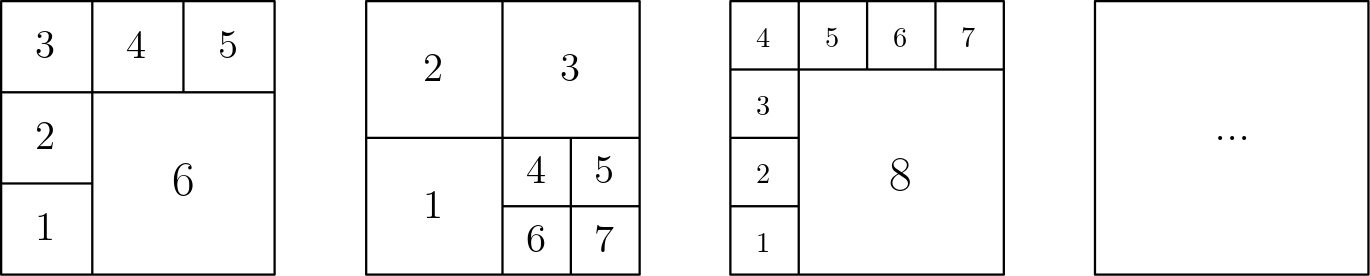
\includegraphics[width = 0.7\textwidth]{3_1.png}
	\caption{Разделение квадратов на $n$ более маленьких квадратиков}
	\label{3_1}
\end{figure}

Пусть $\leq n$ - уже доказано $\Rightarrow$ 

\begin{figure}[H]
	\centering
	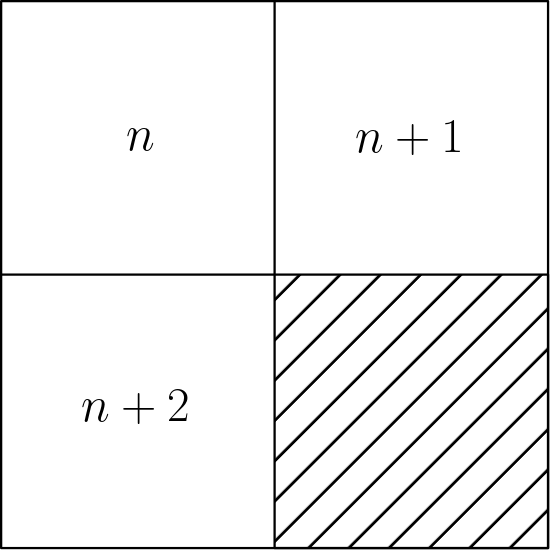
\includegraphics[width = 0.25\textwidth]{3_2.png}
	\caption{Разбиение квадрата на $n+1$ часть}
	\label{3_2}
\end{figure}
По рисунку: для закрашенной части как $n-2$ уже доказано $\Rightarrow$  разделили по индукции на $n+1$ часть.
\end{proof}

\section*{Основная теорема арифметики}

\begin{theorem}
	Всякое натуральное число $> 1$ либо является простым, либо раскладывается в произведение простых, единственным образо с точностью до порядка множителей.
\end{theorem}
\begin{proof}
	\textbf{(существование)} \uline{База}: $n=2$ - доказано.\\
	\uline{Шаг}: пусть для $\leq n$ - доказано, докажем для $n+1$: $n+1$ - простое $\Rightarrow$ ok, $n+1$ - составное $\Rightarrow n + 1 = n_1 \cdot n_2, n+1 > n_1 > 1, \, n+1 > n_2 > 1 \Rightarrow n_1 \leq n,\, n_2 \leq n \Rightarrow$ по индукции, либо $n_1\cdot n_2$ - простые, либо раскладываются на простые множители $\Rightarrow$ ok. 
\end{proof}

\begin{prop}
	Полная математическая индукция $\Leftrightarrow$ обычная математическая индукция.
\end{prop}
\begin{proof}
	\uwave{обычная МИ} $\Rightarrow$ \uwave{полная МИ}: очевидно, ok.\\
	\uwave{полная МИ} $\Rightarrow$ \uwave{обычная МИ}: $A_1$ - истина, $(A_1, \dotsc, A_n)$ - истина $\Rightarrow A_{n+1}$ - истина.\\ 
	Пусть $B_n = \{\, A_1, \dotsc, A_n$ - все истины$\,\} \Rightarrow A_1$ - истина $\Leftrightarrow B_1$ - истина.\\
	$\big( (A_1, \dotsc, A_n) \Rightarrow A_{n+1}  \big) \Leftrightarrow (B_n \Rightarrow B_{n+1})$, то есть к $B_n$ применяем обычную индукцию и $B_{n+1}$ - истина, получаем, что все $B_n$ - истинные и все $A_n$ - истинные $\Rightarrow$ ok.
\end{proof}

\section*{Запись полной индукции на языке теории множеств}
Пусть $M \subset \mathbb{N}$. Если $1 \in M$ и $\{\, k \colon k \leq n \,\} \subset M \Rightarrow n+1 \in M$, то $M = \mathbb{N}$.\\ 
Далее используем это как \uwave{аксиому индукции} (АИ).

\begin{theorem}
	Пусть множество $\mathbb{N}$ удовлетворяет аксиомам Пеано (1)-(3) и на $\mathbb{N}$ задано отношение линейного порядка, причем $n \leq n+1$. Тогда (АИ) равносильна существованию в каждом непустом подмножестве наименьшего элемента.
\end{theorem}

\begin{proof}
	($\Rightarrow$)  Пусть $B \subset \mathbb{N}$, $B \neq \varnothing$, предположим противное, что в $B$ не существует такого элемента. $M = \mathbb{N} \setminus B \Rightarrow 1 \in M$, так как если $1 \in B \Rightarrow$ наименьшее, $\{\, k \colon k \leq n\,\} \subset M \Rightarrow n + 1 \in M$, иначе оно - наименьшее в $B$, так как все остальное, что меньше в $M \Rightarrow$ по АИ $M = \mathbb{N} \Rightarrow$ поскольку $B \neq \varnothing$ получаем противоречие.
	
	($\Leftarrow$) Пусть $M \subset \mathbb{N}\colon 1\in M$, $\{\, k \colon k \leq n \,\} \subset M \Rightarrow n+1 \in M$, хотим $M = \mathbb{N}$. Пусть $\mathbb{N}\setminus M \neq \varnothing$, $n \in \mathbb{N}\setminus M$, $n$ - наименьшее. $n \neq 1$ так как $1 \in M \Rightarrow$ по АП $n = m+1,\, \{\, k \colon k \leq m \,\} \subset M \Rightarrow m + 1\in M$ по условию на $M$ и поскольку $n$ - наименьшее, все что меньше не лежат в $\mathbb{N} \setminus M \Rightarrow$ противоречие $\Rightarrow \mathbb{N} \setminus M = \varnothing \Rightarrow \mathbb{N} = M$.
\end{proof}

Все переносится на $\mathbb{Z}$, после установки для $\mathbb{N}$, точно также они переносятся с $\mathbb{Z}$ на $\mathbb{Q}$:\\
 $\dfrac{m}{n} \leq \dfrac{p}{q} \Leftrightarrow mq \leq np;\, n, q \in \mathbb{N}, \, m, p \in \mathbb{Z}$.

\section*{Операции со множествами}

\begin{enumerate}[label={(\arabic*)}]
	\item Объединение: $A \cup B = \{\, x \mid x \in A \vee x \in B \,\}$;
	\item Пересечение: $A \cap B = \{\, x \mid x \in A \wedge x \in B \,\}$;
	\item Объединение произвольного набора множеств: $\bigcup\limits_\alpha A_\alpha = \{\, x \mid \exists \alpha \colon x \in A_\alpha \,\}$;
	\item Пересечение произвольного набора множеств: $\bigcap\limits_\alpha A_\alpha = \{\, x \mid x \in A_\alpha, \forall \alpha \,\}$;
	\item Разность множеств: $A \setminus B = \{\, x \mid x \in A \wedge x \notin B \,\}$;
\end{enumerate}

Множества удобно визуализировать с помощью диаграмм Эйлера.
\begin{exrc}
	Доказать, что таких диаграмм нет для 4-ех и более множеств (кругов).
\end{exrc}
\begin{figure}[H]
	\centering
	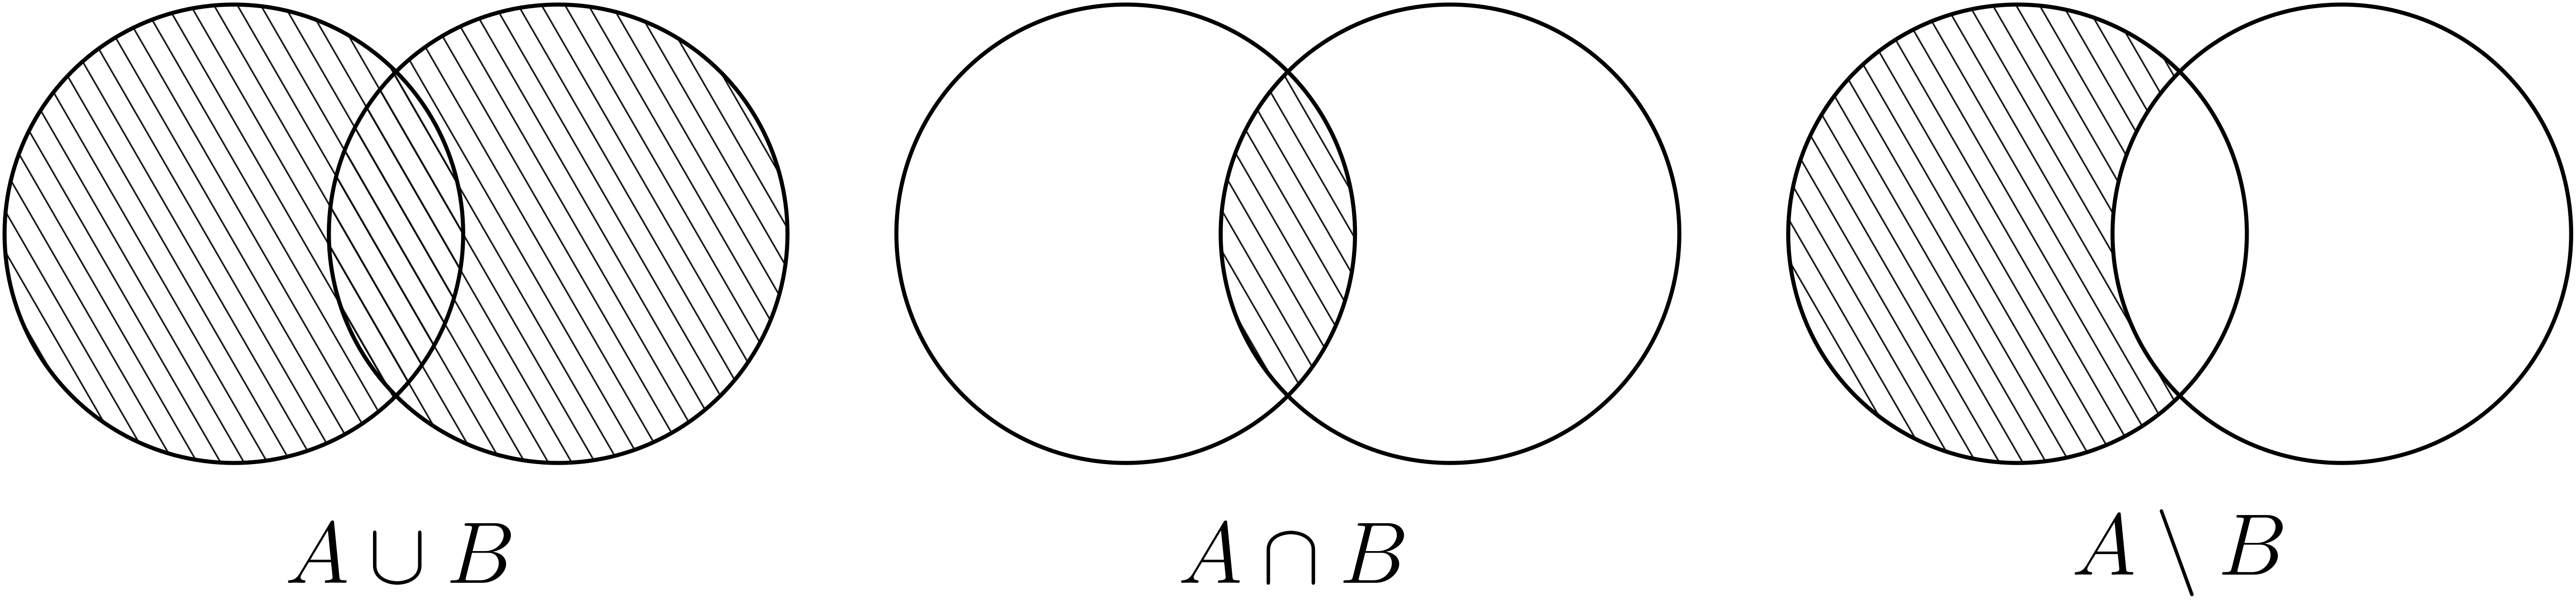
\includegraphics[width = 0.75\textwidth]{3_3.png}
	\caption{Диаграммы Эйлера (круги Эйлера)}
	\label{3_3}
\end{figure}

\subsection*{Свойства операций:}

\begin{enumerate}[label={(\Roman*)}]
	\item $A \cap B = B \cap A$, $A \cup B = B \cup A$;
	\item $A \cap (B \cap C) = (A \cap B) \cap C$, $A \cup (B \cup C) = (A \cup B) \cup C$;
	\item $A \cap (B \cup C) = (A \cap B) \cup (A \cap C)$, $A \cup (B \cap C) = (A \cup B) \cap (A \cup C)$;
	\item \uwave{Формулы Моргана}: $C \setminus (A\cup B) = (C \setminus A) \cap (C\setminus B)$, $C \setminus (A\cap B) = (C \setminus A) \cup (C\setminus B)$;
	\item \uwave{Формулы Моргана в общем случае}: $C \setminus \bigcup\limits_\alpha A_\alpha = \bigcap\limits_\alpha (C \setminus A_\alpha)$, $C \setminus \bigcap\limits_\alpha A_\alpha = \bigcup\limits_\alpha (C \setminus A_\alpha)$;
\end{enumerate}
	
\begin{proof}
(III) (Графический способ) - используем диаграмы Эйлера, чтобы убедиться в справедливости формул.
\begin{figure}[H]
	\centering
	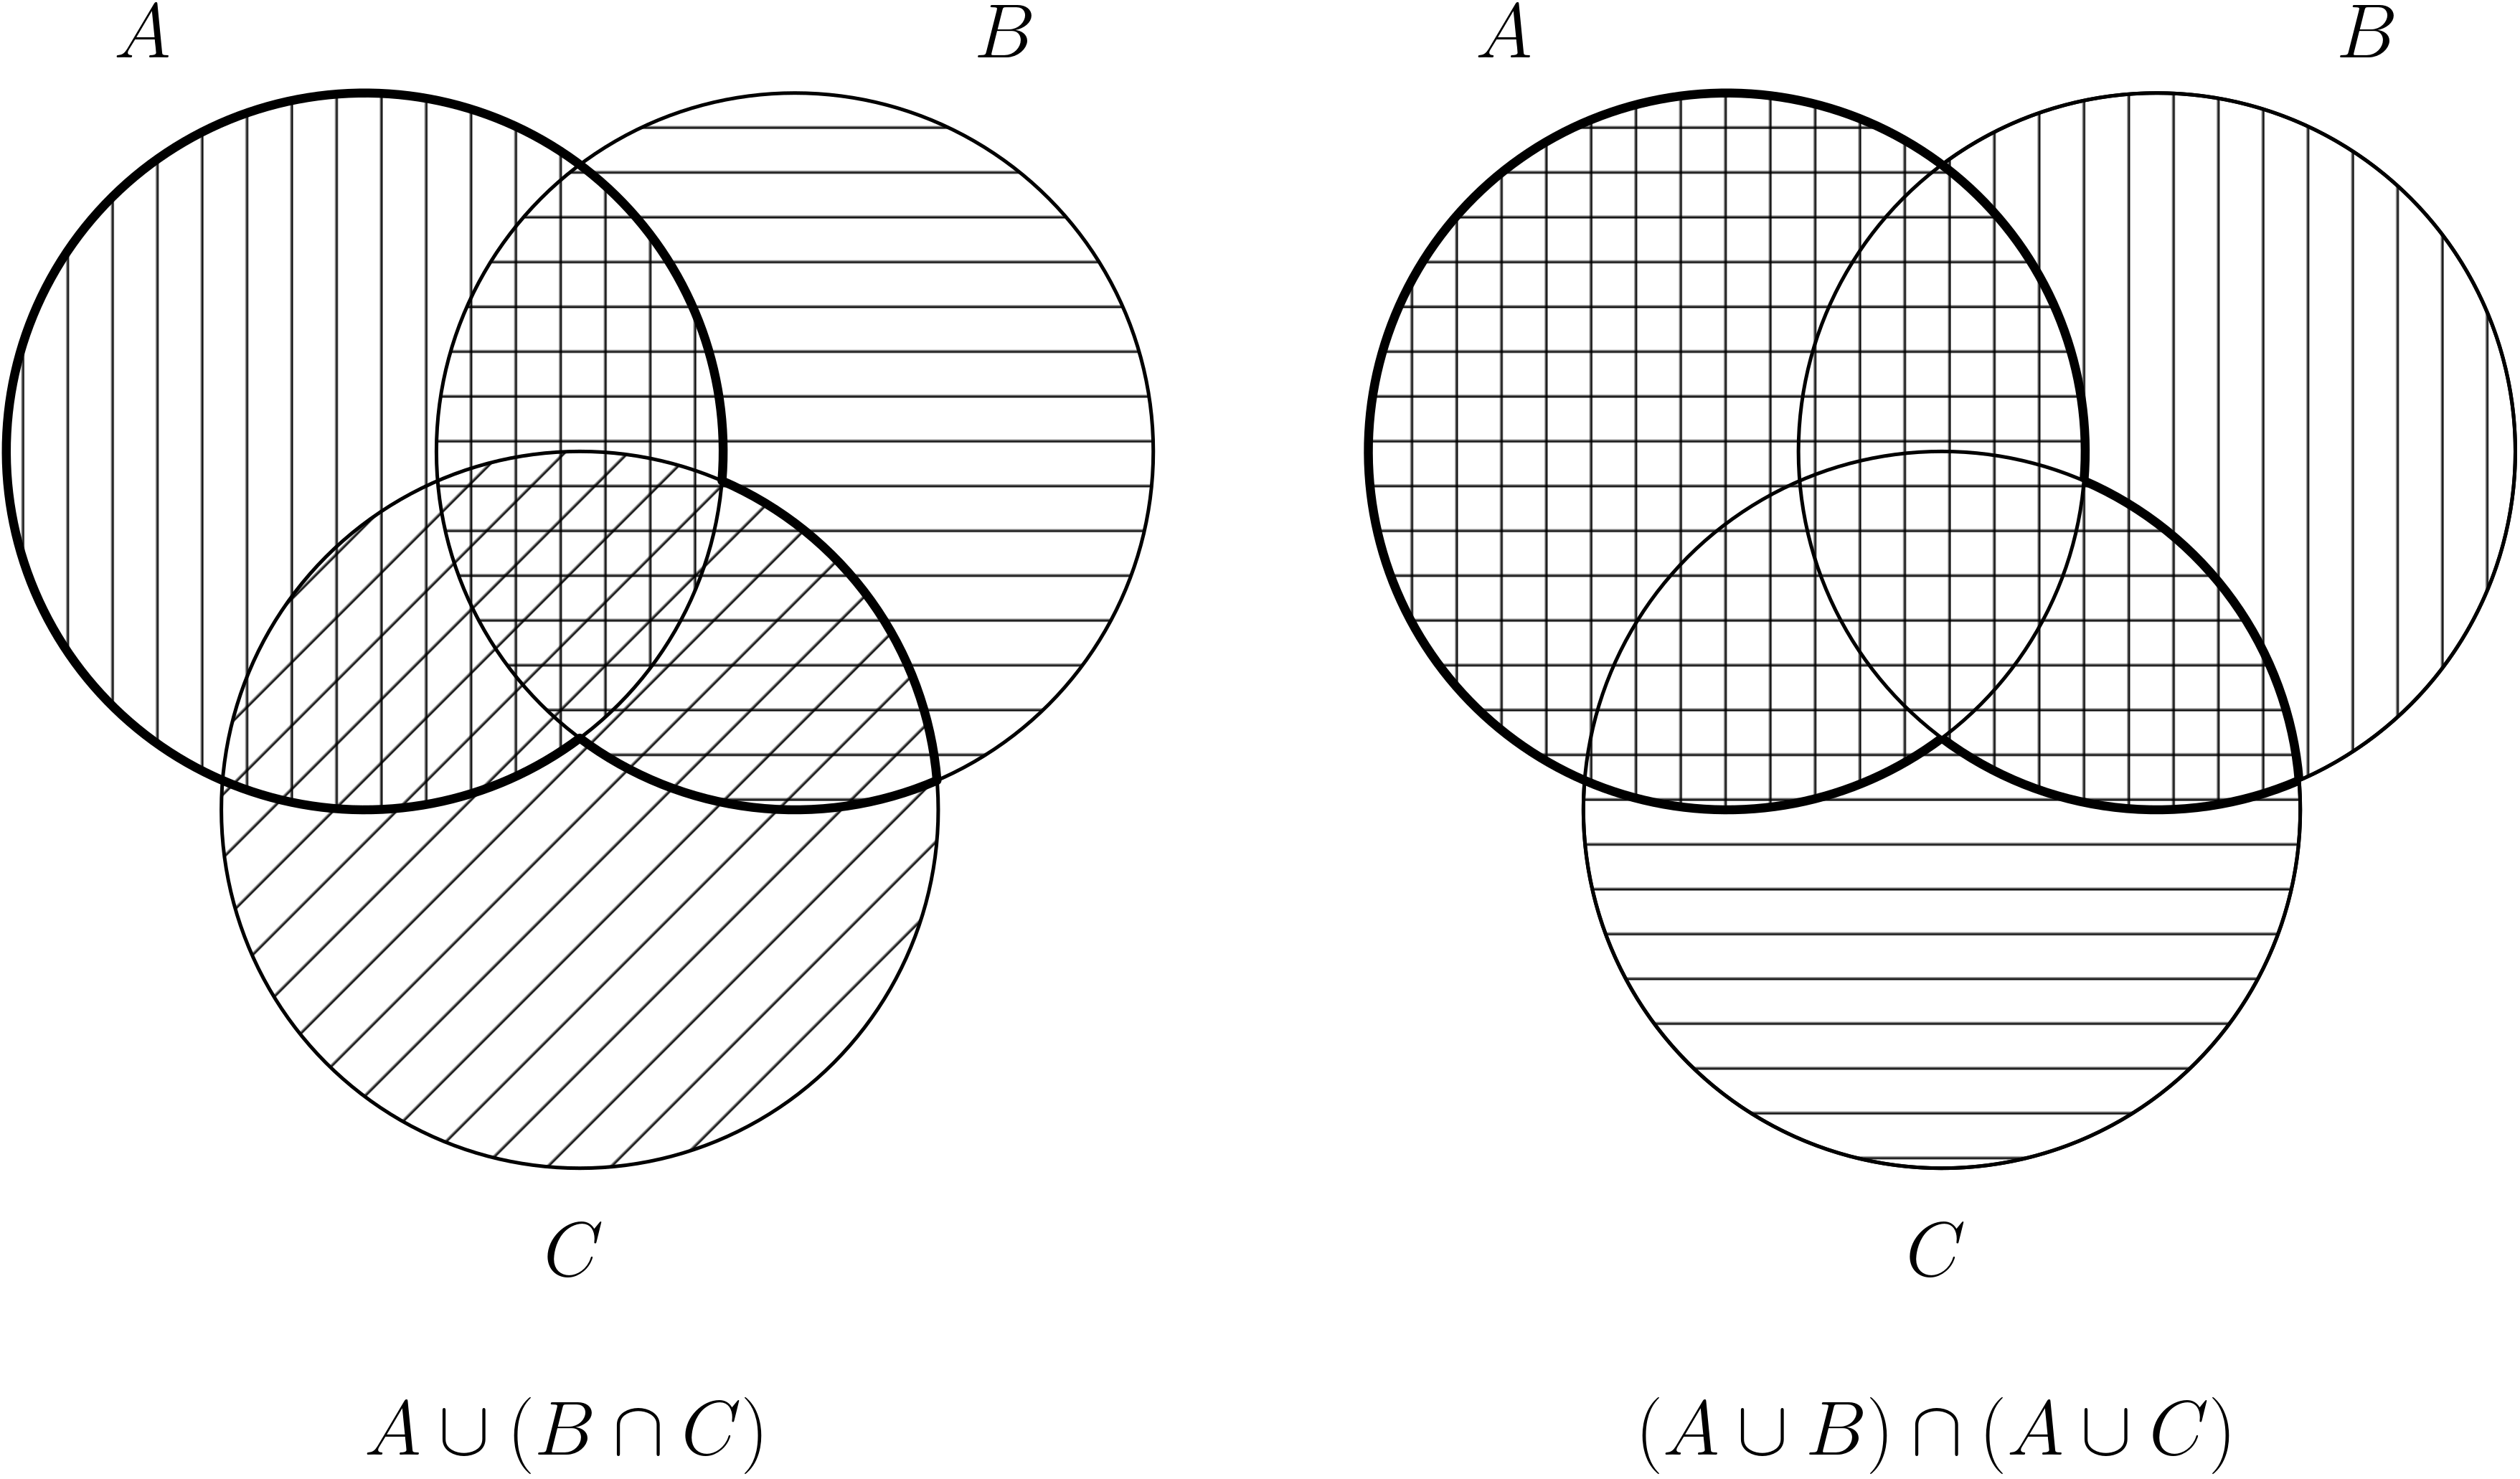
\includegraphics[width = 0.7\textwidth]{3_4.png}
	\caption{Диаграммы Эйлера для свойства (III)}
	\label{fig:3_4}
\end{figure}

\uwave{Формально}: $x \in A \cup (B\cap C) \Leftrightarrow x\in A \vee x \in (B \cap C) \Leftrightarrow x \in A \vee (x\in B \wedge x\in C) \Leftrightarrow$\\
 $\Leftrightarrow (x \in A \vee x\in B) \wedge (x\in A \vee x \in C) \Leftrightarrow x \in (A\cup B)\wedge x \in (A \cup C) \Leftrightarrow x \in (A\cup B) \cap (A \cup C)$.

(V): $x \in C \setminus \bigcup\limits_\alpha A_\alpha \Leftrightarrow x \in C \wedge x \notin \bigcup\limits_\alpha A_\alpha \Leftrightarrow x \in C \wedge (x \notin A_\alpha, \forall \alpha) \Leftrightarrow x \in C \setminus A_\alpha, \forall \alpha \Leftrightarrow x \in \bigcap\limits_\alpha (C \setminus A_\alpha)$.
\end{proof}
	
\end{document}